% GNUPLOT: LaTeX picture with Postscript
\begingroup
  % Encoding inside the plot.  In the header of your document, this encoding
  % should to defined, e.g., by using
  % \usepackage[latin1,<other encodings>]{inputenc}
  \inputencoding{latin1}%
  \makeatletter
  \providecommand\color[2][]{%
    \GenericError{(gnuplot) \space\space\space\@spaces}{%
      Package color not loaded in conjunction with
      terminal option `colourtext'%
    }{See the gnuplot documentation for explanation.%
    }{Either use 'blacktext' in gnuplot or load the package
      color.sty in LaTeX.}%
    \renewcommand\color[2][]{}%
  }%
  \providecommand\includegraphics[2][]{%
    \GenericError{(gnuplot) \space\space\space\@spaces}{%
      Package graphicx or graphics not loaded%
    }{See the gnuplot documentation for explanation.%
    }{The gnuplot epslatex terminal needs graphicx.sty or graphics.sty.}%
    \renewcommand\includegraphics[2][]{}%
  }%
  \providecommand\rotatebox[2]{#2}%
  \@ifundefined{ifGPcolor}{%
    \newif\ifGPcolor
    \GPcolortrue
  }{}%
  \@ifundefined{ifGPblacktext}{%
    \newif\ifGPblacktext
    \GPblacktextfalse
  }{}%
  % define a \g@addto@macro without @ in the name:
  \let\gplgaddtomacro\g@addto@macro
  % define empty templates for all commands taking text:
  \gdef\gplbacktext{}%
  \gdef\gplfronttext{}%
  \makeatother
  \ifGPblacktext
    % no textcolor at all
    \def\colorrgb#1{}%
    \def\colorgray#1{}%
  \else
    % gray or color?
    \ifGPcolor
      \def\colorrgb#1{\color[rgb]{#1}}%
      \def\colorgray#1{\color[gray]{#1}}%
      \expandafter\def\csname LTw\endcsname{\color{white}}%
      \expandafter\def\csname LTb\endcsname{\color{black}}%
      \expandafter\def\csname LTa\endcsname{\color{black}}%
      \expandafter\def\csname LT0\endcsname{\color[rgb]{1,0,0}}%
      \expandafter\def\csname LT1\endcsname{\color[rgb]{0,1,0}}%
      \expandafter\def\csname LT2\endcsname{\color[rgb]{0,0,1}}%
      \expandafter\def\csname LT3\endcsname{\color[rgb]{1,0,1}}%
      \expandafter\def\csname LT4\endcsname{\color[rgb]{0,1,1}}%
      \expandafter\def\csname LT5\endcsname{\color[rgb]{1,1,0}}%
      \expandafter\def\csname LT6\endcsname{\color[rgb]{0,0,0}}%
      \expandafter\def\csname LT7\endcsname{\color[rgb]{1,0.3,0}}%
      \expandafter\def\csname LT8\endcsname{\color[rgb]{0.5,0.5,0.5}}%
    \else
      % gray
      \def\colorrgb#1{\color{black}}%
      \def\colorgray#1{\color[gray]{#1}}%
      \expandafter\def\csname LTw\endcsname{\color{white}}%
      \expandafter\def\csname LTb\endcsname{\color{black}}%
      \expandafter\def\csname LTa\endcsname{\color{black}}%
      \expandafter\def\csname LT0\endcsname{\color{black}}%
      \expandafter\def\csname LT1\endcsname{\color{black}}%
      \expandafter\def\csname LT2\endcsname{\color{black}}%
      \expandafter\def\csname LT3\endcsname{\color{black}}%
      \expandafter\def\csname LT4\endcsname{\color{black}}%
      \expandafter\def\csname LT5\endcsname{\color{black}}%
      \expandafter\def\csname LT6\endcsname{\color{black}}%
      \expandafter\def\csname LT7\endcsname{\color{black}}%
      \expandafter\def\csname LT8\endcsname{\color{black}}%
    \fi
  \fi
    \setlength{\unitlength}{0.0500bp}%
    \ifx\gptboxheight\undefined%
      \newlength{\gptboxheight}%
      \newlength{\gptboxwidth}%
      \newsavebox{\gptboxtext}%
    \fi%
    \setlength{\fboxrule}{0.5pt}%
    \setlength{\fboxsep}{1pt}%
\begin{picture}(8502.00,5102.00)%
    \gplgaddtomacro\gplbacktext{%
      \csname LTb\endcsname%%
      \put(814,704){\makebox(0,0)[r]{\strut{}$1.2$}}%
      \put(814,1168){\makebox(0,0)[r]{\strut{}$1.3$}}%
      \put(814,1632){\makebox(0,0)[r]{\strut{}$1.4$}}%
      \put(814,2096){\makebox(0,0)[r]{\strut{}$1.5$}}%
      \put(814,2560){\makebox(0,0)[r]{\strut{}$1.6$}}%
      \put(814,3025){\makebox(0,0)[r]{\strut{}$1.7$}}%
      \put(814,3489){\makebox(0,0)[r]{\strut{}$1.8$}}%
      \put(814,3953){\makebox(0,0)[r]{\strut{}$1.9$}}%
      \put(814,4417){\makebox(0,0)[r]{\strut{}$2$}}%
      \put(814,4881){\makebox(0,0)[r]{\strut{}$2.1$}}%
      \put(946,484){\makebox(0,0){\strut{}$-0.3$}}%
      \put(1841,484){\makebox(0,0){\strut{}$-0.2$}}%
      \put(2736,484){\makebox(0,0){\strut{}$-0.1$}}%
      \put(3631,484){\makebox(0,0){\strut{}$0$}}%
      \put(4526,484){\makebox(0,0){\strut{}$0.1$}}%
      \put(5420,484){\makebox(0,0){\strut{}$0.2$}}%
      \put(6315,484){\makebox(0,0){\strut{}$0.3$}}%
      \put(7210,484){\makebox(0,0){\strut{}$0.4$}}%
      \put(8105,484){\makebox(0,0){\strut{}$0.5$}}%
    }%
    \gplgaddtomacro\gplfronttext{%
      \csname LTb\endcsname%%
      \put(198,2792){\rotatebox{-270}{\makebox(0,0){\strut{}$\frac{\langle L^4 \rangle}{\langle L^2 \rangle^2}$}}}%
      \put(4525,154){\makebox(0,0){\strut{}$\frac{\beta - \beta_c}{\beta_c}N_\sigma^{1/\nu}$}}%
      \csname LTb\endcsname%%
      \put(7118,4708){\makebox(0,0)[r]{\strut{}$N_\sigma =\  8$}}%
      \csname LTb\endcsname%%
      \put(7118,4488){\makebox(0,0)[r]{\strut{}$N_\sigma =\  9$}}%
      \csname LTb\endcsname%%
      \put(7118,4268){\makebox(0,0)[r]{\strut{}$N_\sigma = 10$}}%
      \csname LTb\endcsname%%
      \put(7118,4048){\makebox(0,0)[r]{\strut{}$N_\sigma = 11$}}%
      \csname LTb\endcsname%%
      \put(7118,3828){\makebox(0,0)[r]{\strut{}$N_\sigma = 12$}}%
      \csname LTb\endcsname%%
      \put(7118,3608){\makebox(0,0)[r]{\strut{}$N_\sigma = 13$}}%
      \csname LTb\endcsname%%
      \put(7118,3388){\makebox(0,0)[r]{\strut{}$N_\sigma = 14$}}%
      \csname LTb\endcsname%%
      \put(7118,3168){\makebox(0,0)[r]{\strut{}$N_\sigma = 15$}}%
      \csname LTb\endcsname%%
      \put(7118,2948){\makebox(0,0)[r]{\strut{}$N_\sigma = 16$}}%
      \csname LTb\endcsname%%
      \put(7118,2728){\makebox(0,0)[r]{\strut{}angepasste Parabel}}%
      \csname LTb\endcsname%%
      \put(1393,1168){\makebox(0,0)[l]{\strut{}$\beta_c=\num{2.2977+-0.0002}\qquad\nu=\num{0.64+-0.02}$}}%
      \put(1393,1632){\makebox(0,0)[l]{\strut{}reduziertes $\chi^2 = \num{1.05}$}}%
    }%
    \gplbacktext
    \put(0,0){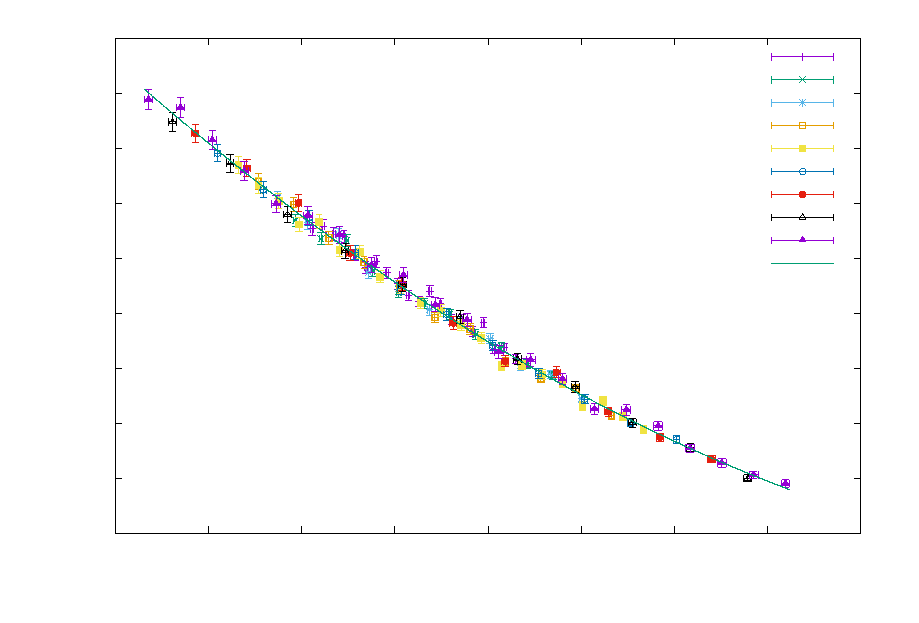
\includegraphics{./fin_size_scaling}}%
    \gplfronttext
  \end{picture}%
\endgroup
